\chapter{Конструкторский раздел}
\label{cha:design}
\section{База данных}
\subsection{Структура базы данных}
В базе данных будут представлены следующие классы сущностей.
\begin{itemize}
\item Films -- класс фильмов
\item Person -- класс людей
\begin{itemize}
\item Actor -- класс актёров
\item Director -- класс режисёров
\end{itemize}
\item Country -- класс страны
\end{itemize}
Также ввиде класса будут представлены жанры. 
У каждого класса есть набор связей.
\begin{itemize}
\item is\_a - связь между подклассом и классом
\item include - связь включения между классом и подклассом 
\item Acted - связь между человеком и фильмом где он снимался
\item Directed - связь между режисёром и режисируемым фильмом 
\item InvolveAsActor - связь между фильмом и актёром
\item InvolveAsDirector - связь между фильмом и режиссёром
\item ProductionCountries - связь между фильмом и выпустившей его страной 
\item Products - связь между страной и выпущенным фильмом
\end{itemize}
Свойства же в OWL определяются как отдельные связи с указанием домена.
\begin{table}[ht]
  \caption{Свойства объектов}
  \begin{tabular}{|c|c|c|}
  \hline
    Имя    & Домен & Определение\\
  \hline
  system\_name & Thing & системное имя объекта\\
  \hline
  Name & Thing & имя объекта\\
  \hline
  DateOfBirthday  & Person   & дата рождения человека\\  
  \hline
  DateOfRelease & Films & Год выпуска фильма \\
  \hline
  \end{tabular}
  \label{tab:tabular}
\end{table}
\subsection{Алгоритм заполнения базы данных}
Так как для семантической сети нам необходима некоторая структуризация данных, нам необходимо установить между вершинами дополнительные связи и присвоить их дополнительным классам. Так как из предыдущей части видно, что одна связь может подразумевать более общую связь и обратную связь.
Для восстановления дополнительных связей и классов было решено действовать по следующему алгоритму.
\begin{enumerate}
\item Загрузить данные с сайта
\item Сохранить данные в OWL формате по подготовленной схеме.
\item Выгрузить данные из OWL дополняя все связи и классы согласно схеме OWL.
\end{enumerate}
Таким образом используя OWL мы получаем возможность обобщать и интерпритировать некоторые данные изначально факты.
\subsection{Сбор данных об онтологии}
Для большинства операций с базой система должна иметь доступ к информации об имеющихся в системе классах и их свойствах. 
Для этого входе обработки онтологии о загруженном классе записываются следующие данные:
\begin{itemize}
\item Системное имя объекта - уникальный идентификатор объекта в системе
\item Базовые классы объекта
\item 
\end{itemize}
О загруженной связи записываются следующие данные:
\begin{itemize}
\item системное имя
\item Область определения
\item Область значений
\end{itemize}
Все эти данные сохраняются для последующего использования в системе.
\subsection{Перенос онтологии в базу данных}
Из-за различных сущностей, которыми представленны данные в онтологии и в базе данных, требуется ввести некоторые правила перевода сущностей.
\begin{center}
\begin{figure}[!h]
  \centering
  \includegraphics[width=\textwidth]{./inc/diag/02_A0.png}
  \caption{Перенос онтологии в базу данных}
  \label{fig:fig01}
\end{figure}
\end{center}
Представленный порядок действий обусловлен зависимостью сущностей. Так связь или свойства вершины не могут быть созданы без вершины, к которой они должны быть применены. 
Также были определены следующие правила переноса. 
\begin{itemize}
\item Классы представляются в базе данных как вершины
\item Объекты представляются в базе данных как вершины
\item Связи с областью значений принадлежащей классам онтологии, устанавливаются у классов области опредения и классов области значений
\item Связи применяются к соответствующим вершинам
\item Связи с областью значений не принадлежащей классам онтологии применяются к соответствующим вершинам(переносятся атрибуты объектов)
\item при помощи связей is\_a и include переносится иерархия объектов 
\end{itemize}
\section{Компрьютерная лингвистика}
\subsection{Синтаксическое дерево}
Синтаксическое дерево - граф показывающий зависимость между словами, полученный в ходе синтаксического анализа. 
\begin{figure}[!h]
  \centering
  \includegraphics[scale = 0.5]{./inc/synt_tree.png}
  \caption{Синтаксическое дерево}
  \label{fig:fig04}
\end{figure}
Узлами графа являются слова, рёбрами является связь между этими словами.
\subsection{Анализ синтаксического дерева}
В данной работе используется следующий алгоритм извлечения данных. 
\begin{enumerate}
\item Происходит обход синтаксического дерева
\item Вершины нормализуются. Входе этого этапа слова приводятся в свою нормальную форму по падежу, роду и склонению.
\item Удаляются игнорируемые токены
\item Данные переводятся во внутреннее представление программы
\end{enumerate}
Данный алгоритм позволяет извлекать данные при наличии явных связей между объектами, однако стоит помнить, что существует множество ситуаций, когда связи в синтаксическом дереве нет. В таких ситуациях следует провести постобработку результатов предыдущего алгоритма или использовать другой алгоритм.
\section{Запросы на естественном языке}
\subsection{Алгоритм обработки запроса на естественном языке}
Обработка запроса на естественном языке будет происходить в несколько этапов. 
\begin{figure}[!h]
  \centering
  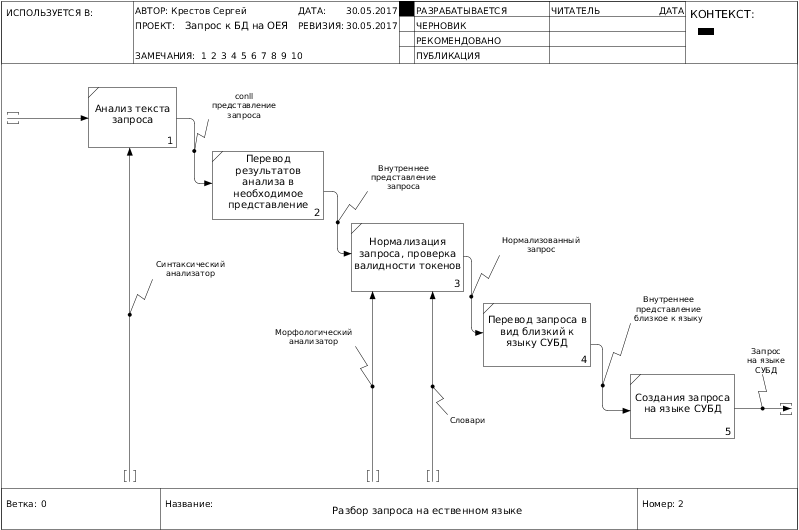
\includegraphics[scale = 0.5]{./first_dia/02_0.png}
  \caption{Синтаксическое дерево}
  \label{fig:fig04}
\end{figure}
В ходе первых этапов данной обработки будет получено некоторое представление об объектах фигурирующих в запросе.  Далее каждому объекту запроса присваивается имя. Это имя будет далее фигурировать в запросе на языке бд, для описания объекта и его связей. За каждой связью также закрепляется имя.
\subsection{Словарь}
Для обеспечения связи слова и сущности базы данных, было принято расширить вышеприведённые описания классов и объектов списком слов, которые могут обозначать эту сущность.
Слово указывается в нормализованном виде. В ходе работы программа загружает описание классов и связей и записывает их в словарь, где ключём выступает нормализованное слово. Если одно слово обозначает несколько сущностей, сущности будут образовывать список. Если сущность может быть обозначена множеством слов, сущность будет добавлена во все ячейки словаря, соответствующие множеству обозначающих её слов.

\subsection{Нормализация дерева}
Дерево, полученное после синтаксического анализа, нельзя использовать для составления запроса по следующим причинам. 
\begin{itemize}
\item Дерево содержит множество элементов не несущих полезной информации на данном этапе развития проекта
\item Элементы дерева в текущем представлении не могут быть использованы для получения связанных с ними объектов,так как форма слова в предложении может отличаться от нормальной, используемой в системе вкачестве ключа.
\end{itemize}
Входе нормализации дерева удаляются элементы определённые как игнорируемые, а оставшиеся элементы приводятся в нормальную форму для последующей обработки.\\
Также на этом этапе происходит сопоставление элементов запроса с соответствующими списками сущностей из словаря. \\
Проводя нормализацию запроса система также проверяет корректность каждого элемента запроса. Если элемент не игнорируется и не содержится в словаре, такой запрос признаётся ошибочным.

\subsection{Алгоритм генерации запроса}
Каждая вершина обрабатывается по следующему алгоритму.
\begin{itemize}
\item Вершине присваивается некоторое имя в запросе
\item Описывается базовый класс вершины
\begin{itemize}
\item Вводится связь is\_a с длинной от нуля до бесконечности исходящая из описываемой вершины 
\item Конечная вершина связи описывается как базовый класс
\end{itemize}
\item Описываются свойства вершины
\item Описываются связи и вершины, задействованные в этих связях
\end{itemize}
Таким образом система учитывает принадлежность системы базовому классу и возможность совпадения запрашиваемого объекта и его базового класса.

\section{Существующие аналоги}
Quepy использует следующие технологии для решения поставленных проблем
\begin{itemize}
\item Анализ запроса\\
Для анализа запроса используются шаблоны, описываемые в коде приложения. Что делает расширение возможностей анализа трудоёмким процессом. 
\item Связь с онтологией\\
Для связи с онтологией предлагается создавать пользовательские классы, которые используются в запросах. Языковое описание классов и связей перенесены в онтологии.
content...
\end{itemize}

\section{План тестирования}
Для тестирования, необходимо выделить определённые классы запросов. Для каждого анализатора выделить классы ошибок и определить поведение системы для этих ошибок.

%%% Local Variables:
%%% mode: latex
%%% TeX-master: "rpz"
%%% End:
